%%%%%%%%%%%%%%%%%%%%%%%%%%%%%%%%%%%%%%%%%%%%%%%%%%%%%%%%%%%%%%%%%%%%%%%%%%%%%%%%%%%%%%%%%%%%%%%%%%%%%%%
% Sablona pro projekty ekonometrickych predmetu                                                     %%%
% Vytvoreno v ramci grantu: Ekonometricke nastroje a techniky v realnych ekonomickych aplikacich    %%%
% Autor: Jakub Bucek (jakubbucek@mail.muni.cz)                                                      %%%
% Pripominky, dotazy, namety smerujte na autora nebo na Daniela Nemce (danek@mail.muni.cz)		    %%%
% Vytvoreno: 1.12.2014                                                                              %%%
%%%%%%%%%%%%%%%%%%%%%%%%%%%%%%%%%%%%%%%%%%%%%%%%%%%%%%%%%%%%%%%%%%%%%%%%%%%%%%%%%%%%%%%%%%%%%%%%%%%%%%%

\documentclass[12pt,a4paper,oneside,final]{article}

%%%%%%%%%%%%%%%%%%%%%%%%%%%%%%%%%%%%%%%%%%%%%%%%%%%%%%%%%%%%%%%%%%%%%%%%%%%%%%%%%%%%%%%%%%%%%%%%%%%%%%%
%%%%%%%%%%%%%%%%%%%%%%%%%%%%%%%%%%%%%% ZAKLADNI NASTAVENI %%%%%%%%%%%%%%%%%%%%%%%%%%%%%%%%%%%%%%%%%%%%%

%% Nastaveni kodovani
\usepackage[utf8]{inputenc} 
\usepackage[IL2]{fontenc} %% fonty vhodne pro sazbu ceskych a slovenskych dokumentu
\usepackage[slovak]{babel}

\usepackage{subcaption}
\usepackage{float}

%% Fonty
\usepackage{mathptmx}  %% volne dostupny font Adobe Times Roman
% \usepackage{bookman}
% \usepackage{charter}
% \usepackage{fourier}
% \usepackage{mathpazo}
% \usepackage{newcent}
% \usepackage{palatino}
% \usepackage{utopia}

%% Baliky potrebne pro sazbu matematiky
\usepackage{amssymb,amsthm,amsmath}
\usepackage{bm}
\usepackage{tabularx} %% vylepsene tabulky

%% Balik nutny pro sablonu
\usepackage{garfield} %% nacteni stylu sablony

%% Vlastní definice
\renewcommand\vec[1]{\ensuremath\boldsymbol{#1}} %% tucne vektory
\newtheorem{veta}{Věta}[section]
\swapnumbers
\theoremstyle{definition}
\newtheorem{definice}{Definice}
\theoremstyle{remark}
\newtheorem*{pozn}{Poznámka}
\numberwithin{equation}{section}

\hyphenation{p-hodnota}
\hyphenation{p-hodnoty}


\usepackage{xparse}
  \NewDocumentCommand{\INTERVALINNARDS}{ m m }{
      #1 {,} #2
 }

\NewDocumentCommand{\interval}{ s m >{\SplitArgument{1}{,}}m m o}{
      \IfBooleanTF{#1}{
          \left#2 \INTERVALINNARDS #3 \right#4
      }{
          \IfValueTF{#5}{
              #5{#2} \INTERVALINNARDS #3 #5{#4}
          }{
              #2 \INTERVALINNARDS #3 #4
          }
      }
  }

%%%%%%%%%%%%%%%%%%%%%%%%%%%%%%%%%%%%%%%%%%%%%%%%%%%%%%%%%%%%%%%%%%%%%%%%%%%%%%%%%%%%%%%%%%%%%%%%%%%%%%%
%%%%%%%%%%%%%%%%%%%%%%%%%%%%%%%%%%%%%%%% TITULNI STRANA %%%%%%%%%%%%%%%%%%%%%%%%%%%%%%%%%%%%%%%%%%%%%%%

\NazevPrace{Modelovanie časových rád z~monitorovacieho systému Hawkular}
\Autor{Bc. Pavol Loffay}
\Univerzita{Masarykova univerzita}
\Fakulta{Fakulta informatiky}
\Obor{Service Science Management Engineering}
\Mail{p.loffay@mail.muni.cz}
\DatumOdevzdani{\today}
\Abstrakt{
 Práca spracováva predikciu časových rád prevzatých z~monitorovacieho systému
 Hawkular\footnote{Dostupné na \url{http://www.hawkular.org}}. Tento systém dokáže
 monitorovať Java aplikácie, alebo fyzický hardvér na ktorom je spustený.
 Z~množiny pozorovaných metrík bola vybratá vyťaženosť Java hromady (heap).
 Pre túto časovú radu boli zostrojené modely: \emph{ARIMA} a~exponenciálne vyhladzovanie.
 Ďalej bola demonštrovaná adaptívna filtrácia, ktorá pomocou algoritmu \emph{LMS}
 vypočítala koeficienty \emph{AR} modelu na generovaných dátach.
}
\KlicovaSlova{Časová rada; ARIMA; LMS; Exponenciálne vyhladzovanie; Hawkular;}
\JELklasifikace{C53}

%%%%%%%%%%%%%%%%%%%%%%%%%%%%%%%%%%%%%%%%%%%%%%%%%%%%%%%%%%%%%%%%%%%%%%%%%%%%%%%%%%%%%%%%%%%%%%%%%%%%%%%
%%%%%%%%%%%%%%%%%%%%%%%%%%%%%%%%%%%%%% ZACATEK DOKUMENTU %%%%%%%%%%%%%%%%%%%%%%%%%%%%%%%%%%%%%%%%%%%%%%

\begin{document}
\VytvorTitulniStranu

\section{Úvod}
Monitorovanie dôležitých biznis aplikácii, medzi ktoré patria napríklad bankové systémy alebo rôzne
servery, na ktorých bežia služby využívané 24/7 je veľmi dôležité. Väčšina
monitorovacích systémov dokáže upozorniť administrátora na vyťaženie pri prekročení
hraničnej hodnoty. V~monitorovacom systéme Hawkular je možné zapnúť predikciu tak, že
administrátor bude upozornený vopred ak by náhodou malo dôjsť k~prekročeniu spomenutej
hraničnej hodnoty. Použité modely časových rád v~systéme Hawkular sú varianty
exponenciálneho vyhladzovania. Modely \emph{ARIMA} nemohli byť použité z~dôvodu nestacionarity dát 
a náročnosti na výpočet\,--\,systém je schopný analyzovať aj niekoľko tisíc modelov naraz. 

Táto práca sa zameria na konštrukciu optimálneho \emph{ARIMA} modelu, ktorý následne porovná
s~exponenciálnym vyhladzovaním, konkrétne Holtovou metódou s~lineárnym trendom. Následne
bude demonštrovaná adaptívna filtrácia. Pre výpočetnú nenáročnosť  bola použitá 
kombinácia exponenciálneho vyhladzovania a
adaptívnej filtrácie v~systéme Hawkular.


\section{Identifikácia ARIMA modelu}
V~tejto kapitole budeme analyticky identifikovať najvhodnejší \emph{ARIMA} model, ktorý následne 
porovnáme s~výsledkom funkcie \texttt{auto.arima} z~balíka \texttt{forecast} v~jazyku
\emph{R}.

Začneme vykreslením časovej rady. Na obrázku \ref{obr:heap} je možné vidieť, že časová rada 
obsahuje mierny lineárny trend, čo indikuje nestacionaritu. Vykreslíme autokorelačnú 
(skrátene \emph{ACF}) a~parciálnu autokorelačnú funkciu (skrátene \emph{PACF}).

\begin{figure}[H] 
    \begin{center}
        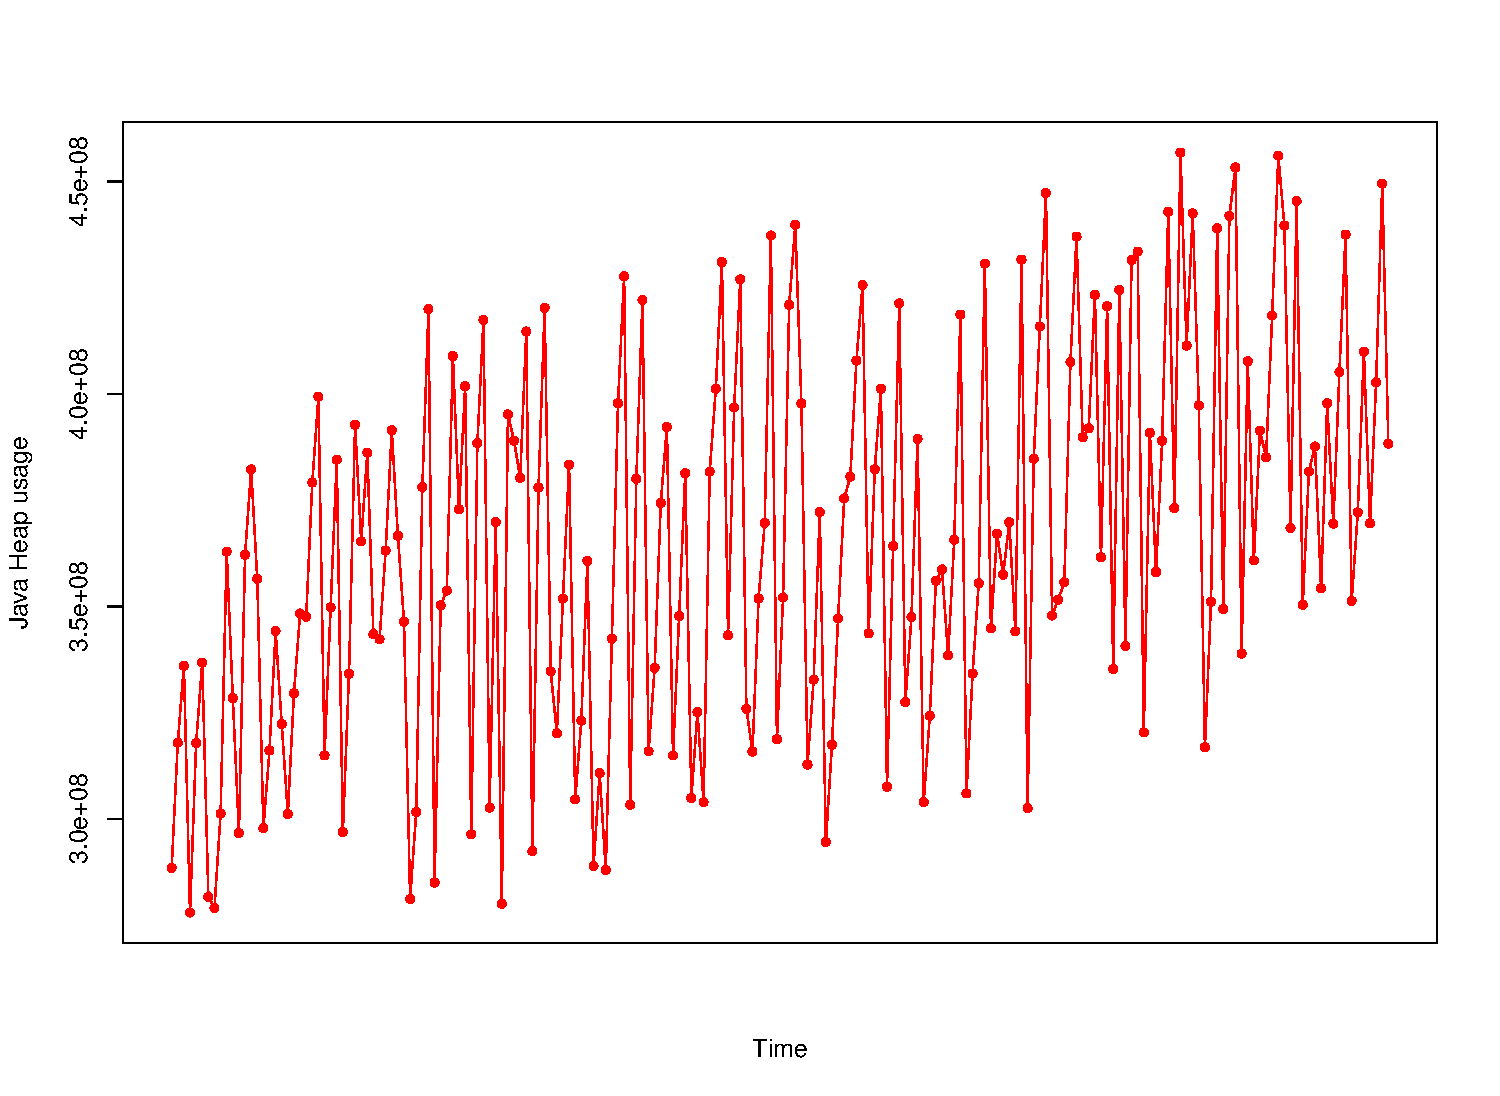
\includegraphics[width=.8\textwidth]{images/heap_series.pdf}
        \caption{Vyťaženosť Java Heap-u v~čase.}
        \label{obr:heap} % unikatni navesti, pomoci ktereho se budeme v textu odvolavat na dany obrazek
    \end{center}
\end{figure}

\begin{figure}[H] \centering
    \begin{subfigure}[b]{0.45\textwidth}
        \centering
        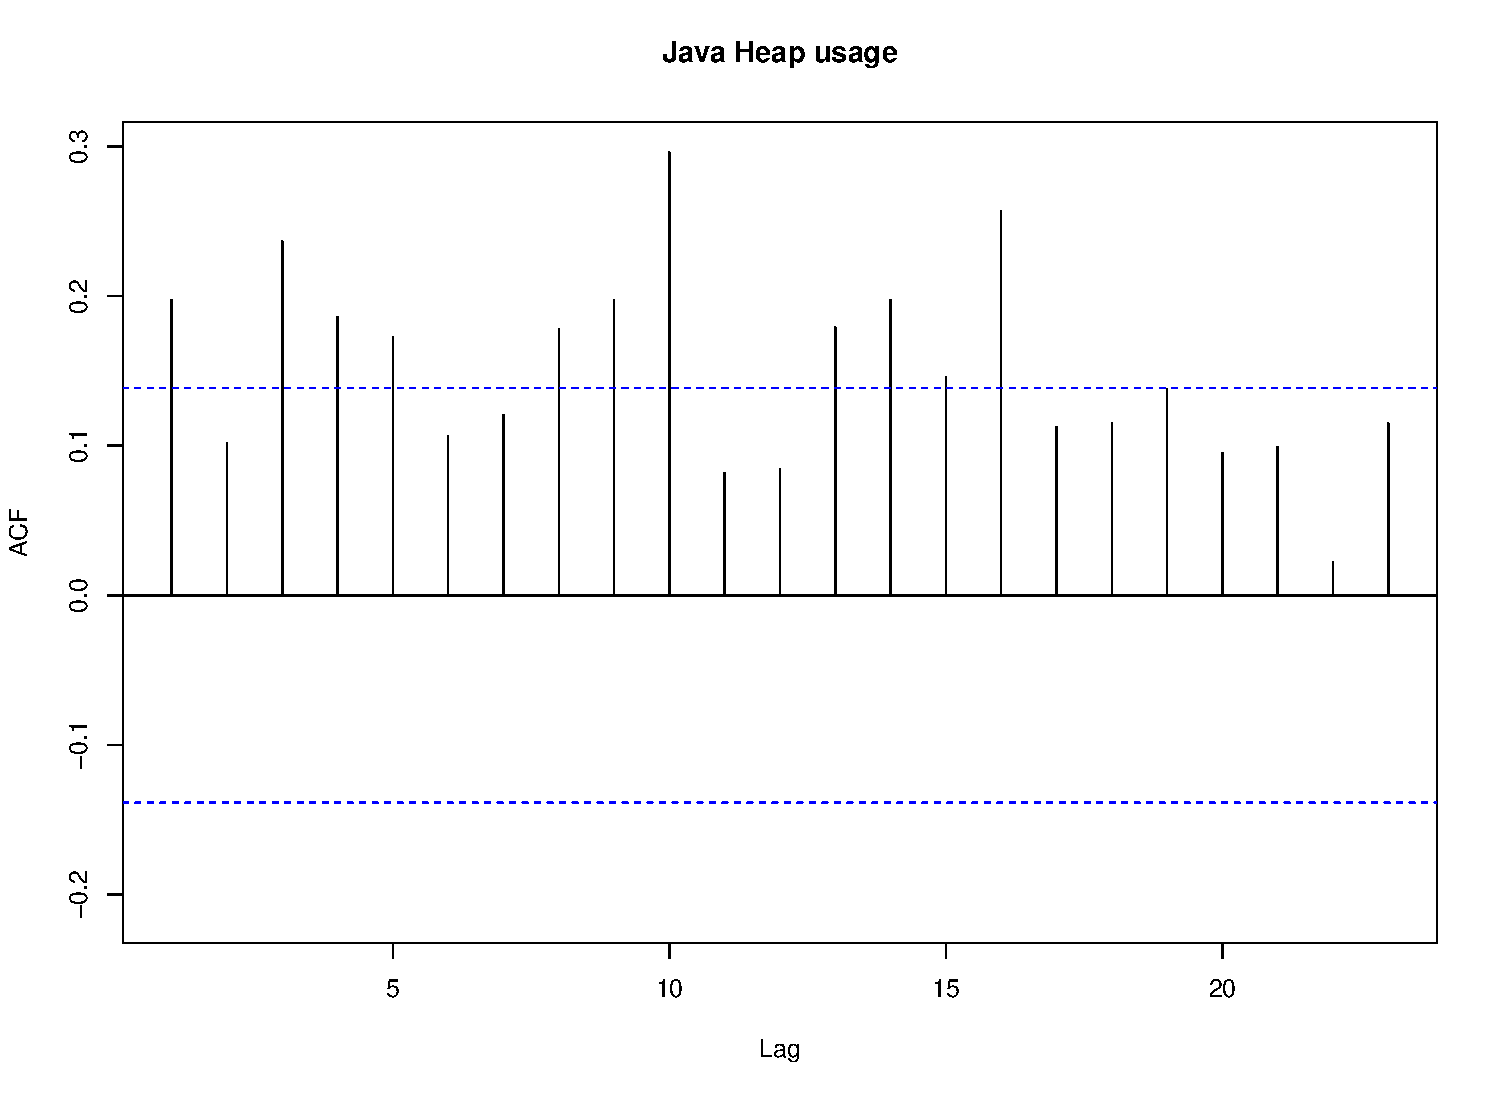
\includegraphics[width=1\linewidth]{images/heap_acf.pdf}
        \caption{Autokorelačná funkcia.}
        \label{obr:heap_acf}
    \end{subfigure}
    \begin{subfigure}[b]{0.45\textwidth}
        \centering
        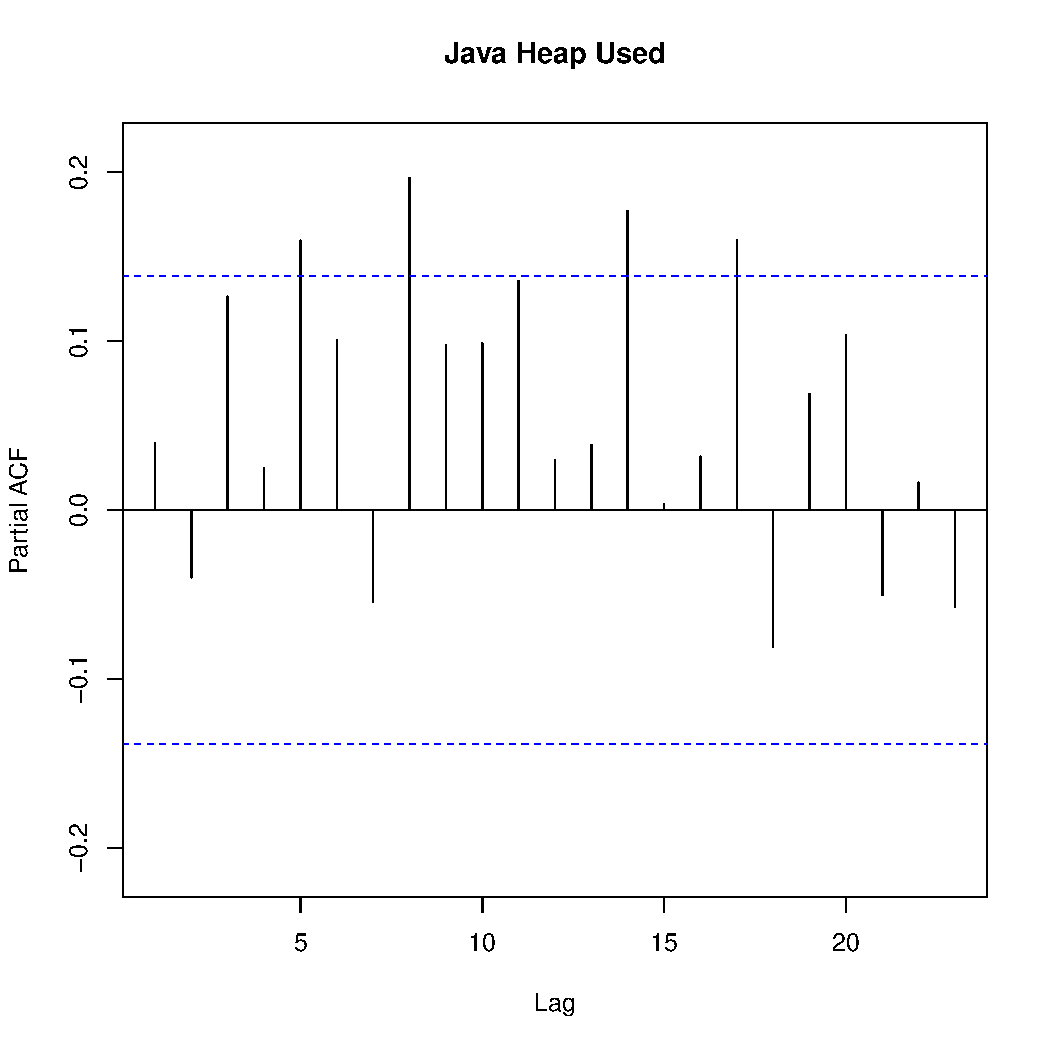
\includegraphics[width=1\linewidth]{images/heap_pacf.pdf}
        \caption{Parciálna autokorelačná funkcia.}
        \label{obr:heap_pacf}
    \end{subfigure}
%    \caption{Parciálna autokorelačná funkcia.}
    %\label{fig:test}
\end{figure}

Z~grafu autokorelačnej funkcie \ref{obr:heap_acf} je vidieť, že hodnoty sú kladné,
relatívne blízko nuly a~neklesajú. 
Na grafe \emph{ACF} taktiež nie sú prítomné periodicky posunuté vysoké hodnoty, 
ktoré by indikovali sezónnosť.
Keďže hodnoty \emph{ACF} so zvyšujúcim oneskorením neklesajú k~nule rozhodli sme sa urobiť
\emph{ADF} test na testovanie stacionarity.

\begin{minipage}{\linewidth}
\begingroup
\fontsize{9pt}{7pt}\selectfont  %ADF
\begin{verbatim}
> adfTest(heap, lags = 0, type='nc');
Title:
 Augmented Dickey-Fuller Test
Test Results:
  PARAMETER:
    Lag Order: 0
  STATISTIC:
    Dickey-Fuller: -1.1436
  P VALUE:
    0.2508 
\end{verbatim}
\endgroup
\end{minipage}

Nulovú hypotézu \emph{ADF} testu o~prítomnosti jednotkového koreňa, na hladine významnosti 0.05
nezamietame. Z~toho vyplýva, že naša časová rada je nestacionárna. Pre dôkladné 
overenie skúsime \emph{KPSS} test, ktorého nulová hypotéza znie, že časová rada je stacionárna.

\begin{minipage}{\linewidth}
\begingroup
\fontsize{9pt}{7pt}\selectfont %KPSS
\begin{verbatim}
> kpss.test(heap);
	KPSS Test for Level Stationarity
data:  heap
KPSS Level = 2.1652, Truncation lag parameter = 3, p-value = 0.01
\end{verbatim}
\endgroup
\end{minipage}

Na hladine významnosti 0.05 by sme nulovú hypotézu zamietli. Oba testy nám ukázali, že časová
rada nie je stacinárna. 
Následne môžeme pomocou \emph{KPSS} testu testovať či je daná časová rada trend stacionárna.

\begin{minipage}{\linewidth}
\begingroup
\fontsize{9pt}{7pt}\selectfont %KPSS Trend
\begin{verbatim}
> kpss.test(heap, null='Trend');
	KPSS Test for Trend Stationarity
data:  heap
KPSS Trend = 0.087693, Truncation lag parameter = 3, p-value = 0.1

> ndiffs(heap)
[1] 1

> diff = diff(heap)
\end{verbatim}
\endgroup
\end{minipage}

Z~výstupu je jasné, že rada je trend stacinárna takže nulovú hypotézu na hladine 0.05
nezamietame.

Časovú radu stacionarizujeme diferencovaním a~pokračujeme vykreslením \emph{ACF} a
\emph{PACF} upravenej časovej rady. 
Významný bod useknutia sa nám v~oboch grafoch \ref{obr:heap_diff_acf_pacf} nepodarilo nájsť. 
To indikuje, že výsledný 
model sa bude skladať z~\emph{AR} aj \emph{MA} zložky. Teraz by sme mali hľadať krivku 
\emph{U}, ktorá od nejakého bodu pripomína krivku v~tvare lineárnych kombinácii klesajúcich
geometrických postupností sinusoid s~geometricky klesajúcimi amplitúdami \cite{cipra}.
Táto krivka v~grafe \emph{ACF} ani \emph{PACF} nie je jednoznačne prítomná. Do modelu sme zahrnuli dve najväčšie 
hodnoty \emph{PACF} (model \emph{AR}) a~jednu \emph{ACF} (model \emph{MA}).
Výsledný model bude má tvar \emph{ARIMA(2,1,1)}.

\begin{figure}[H] \centering
    \begin{subfigure}[b]{0.45\textwidth}
        \centering
        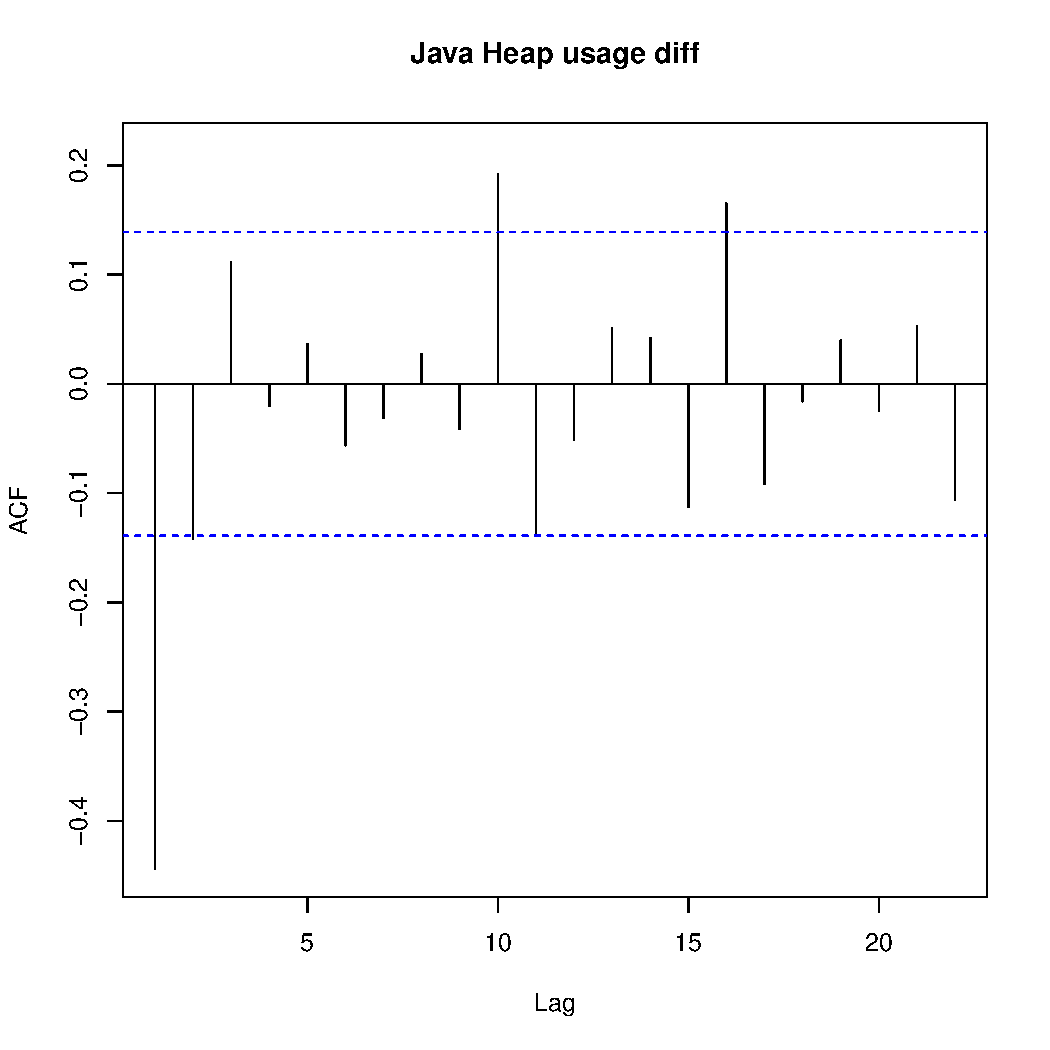
\includegraphics[width=1\linewidth]{images/heap_diff_acf.pdf}
%        \caption{Autokorelačná funkcia diferencovanej rady.}
%        \label{obr:heap_diff_acf}
    \end{subfigure}
    \begin{subfigure}[b]{0.45\textwidth}
        \centering
        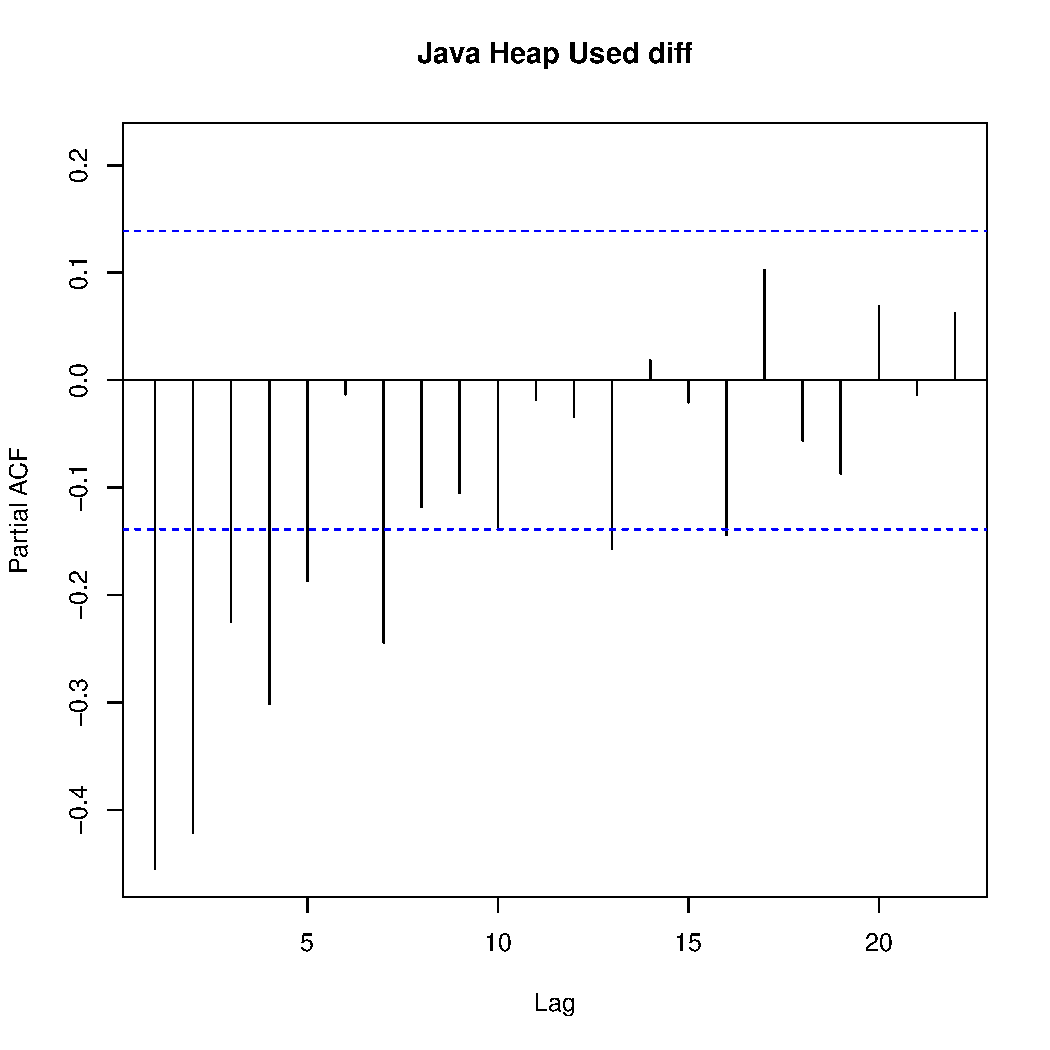
\includegraphics[width=1\linewidth]{images/heap_diff_pacf.pdf}
%        \caption{Parciálna autokorelačná funkcia diferencovanej rady.}
%        \label{obr:heap_diff_pacf}
    \end{subfigure}
    \caption{\emph{ACF} a \emph{PACF} diferencovanej časovej rady.}
    \label{obr:heap_diff_acf_pacf}
\end{figure}

Alternatívny spôsob voľby modelu je pomocou informačných kritérií. Tento spôsob je
vhodný pre plne automatizované spracovanie \cite{cipra} napríklad v~ekonometrických 
softvéroch. K~identifikácii modelu \emph{ARMA(p, q)} sa pristupuje ako k~minimalizácii funkcie
\ref{rov:inf_k}.

\begin{eqnarray} \label{rov:inf_k}
    (\hat{p}, \hat{q}) =arg\ \underset{(k,l)}{min}\ A(k, l)
\end{eqnarray}

\emph{A} je vhodné kritérium pre výpočet ktorého musíme odhadnúť model
\emph{ARMA(k,l)}. Pri minimalizácii postupne inkrementujeme oba parametre k, l.
Informačných kritérií existuje viac. V~tejto práci sme zvolili Akaikovo informačné kritérium:

\begin{eqnarray} \label{rov:aic}
    A(k,l) = AIC(k,l) = ln\hat{\sigma}^{2}_{k,l} + \frac{2(k+l+1)}{n}
\end{eqnarray}

Z~rovnice \ref{rov:aic} je zrejmé, že kritérium penalizuje veľké rády k~a l. 
$\hat{\sigma}^{2}_{k,l}$ je smerodajná odchýlka reziduí modelu. 
Poďme si vypísať niekoľko kandidátov \emph{ARIMA} modelov pomocou príkazu
\texttt{auto.arima}.

\begin{minipage}{\linewidth}
\begingroup
\fontsize{9pt}{7pt}\selectfont %ARIMA
\begin{verbatim}
> auto.arima(diff, approximation=FALSE, trace=TRUE, ic='aic', allowdrift=FALSE)
 ARIMA(2,1,2)                    : 7556.055
 ARIMA(0,1,0)                    : 7696.058
 ARIMA(1,1,0)                    : 7651.407
 ARIMA(0,1,1)                    : 7557.045
 ARIMA(1,1,2)                    : 7560.654
 ARIMA(3,1,2)                    : 7557.714
 ARIMA(2,1,1)                    : 7553.937
 ARIMA(1,1,1)                    : 7557.937
 ARIMA(3,1,1)                    : 7555.879
 ARIMA(2,1,0)                    : 7613.902

 Best model: ARIMA(2,1,1)                    
Series: diff 
ARIMA(2,1,1)                    
Coefficients:
          ar1      ar2      ma1
      -0.0985  -0.1774  -0.9441
s.e.   0.0716   0.0716   0.0199
\end{verbatim}
\endgroup
\end{minipage}

Ako je vidieť funkcia zvolila model \emph{ARIMA(2,1,1)} ktorého \emph{AIC} kritérium bolo najnižšie.
Odhadnutý model môžeme zapísať v~tvare:
\begin{eqnarray} \label{rov:arima_model}
    Y_t = -0.985 Y_{t-1} - 0.1774 Y_{t-2} -0.9441\epsilon_{t-1} + \epsilon_{t}
\end{eqnarray}

Ukázali sme, že je možné skonštruovať správny \emph{ARIMA} model aj analytickým spôsobom. 
Chcel by som však poznamenať, že voľbu modelu je lepšie prenechať overenému 
štatistickému softvéru. 

Po úspešnom odhade rádu modelu by sme chceli spomenúť ako sa počítajú jednotlivé
koeficienty. Pre \emph{AR} model platí, že sa dajú vypočítať pomocou \emph{OLS} alebo Yule\,--\,Walkerových
rovníc \cite{brockwell_ts}. Výpočet koeficientov \emph{MA} modelu je zložitejší a~je 
možný pomocou rekurzívnej Levison\,--\,Durbin metódy.
Odhadom presných parametrov modelu sa v~tejto práci ďalej nebudeme zaoberať.  

Na záver sa pozrieme na rezíduá odhadnutého modelu. Ak sme postupovali správne rezíduá by
mali pripomínať biely šum a~nemali by byť korelované (inakšie by sme ich
vedeli modelovať). Toto tvrdenie si overíme Ljung\,--\,Box testom, ktorého nulová hypotéza
hovorí o~tom, že dáta sú nezávislé distribuované. Z~grafu \ref{obr:heap_resid} môžeme
prehlásiť, že nulovú hypotézu na hladine významnosti 0.05 nezamietame.

Na následujúcich grafoch si vykreslíme rezíduá modelu, ich autokorelačnú funkciu
a~\mbox{p-hodnoty}
pre rôzne oneskorenia Ljung\,--\,Box testu.

\begin{figure}[H] \centering
    \begin{subfigure}{0.55\textwidth}
        \centering
        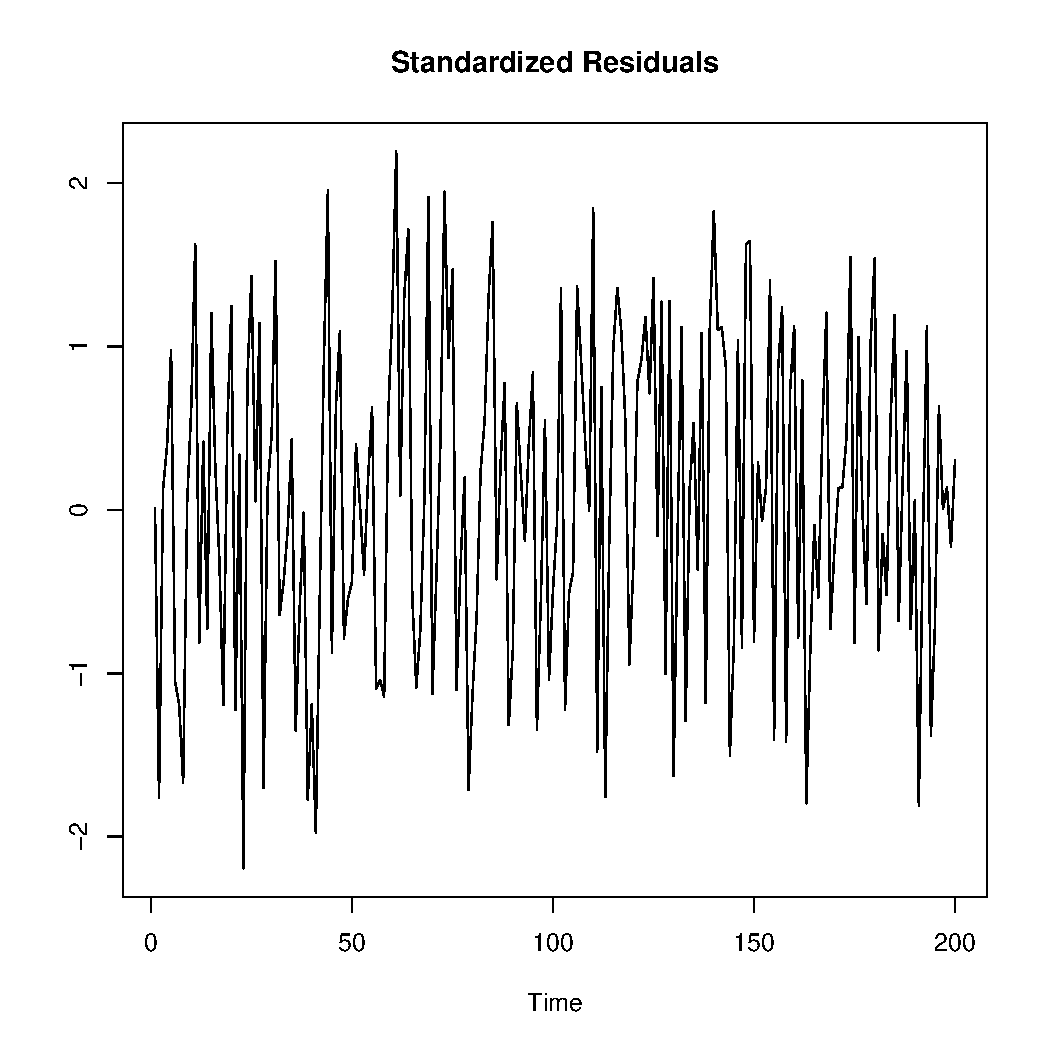
\includegraphics[width=1\linewidth,height=5cm]{images/heap_resid.pdf}
%        \caption{}
        \label{obr:heap_resid_resid}
    \end{subfigure}
    \begin{subfigure}{0.55\textwidth}
        \centering
        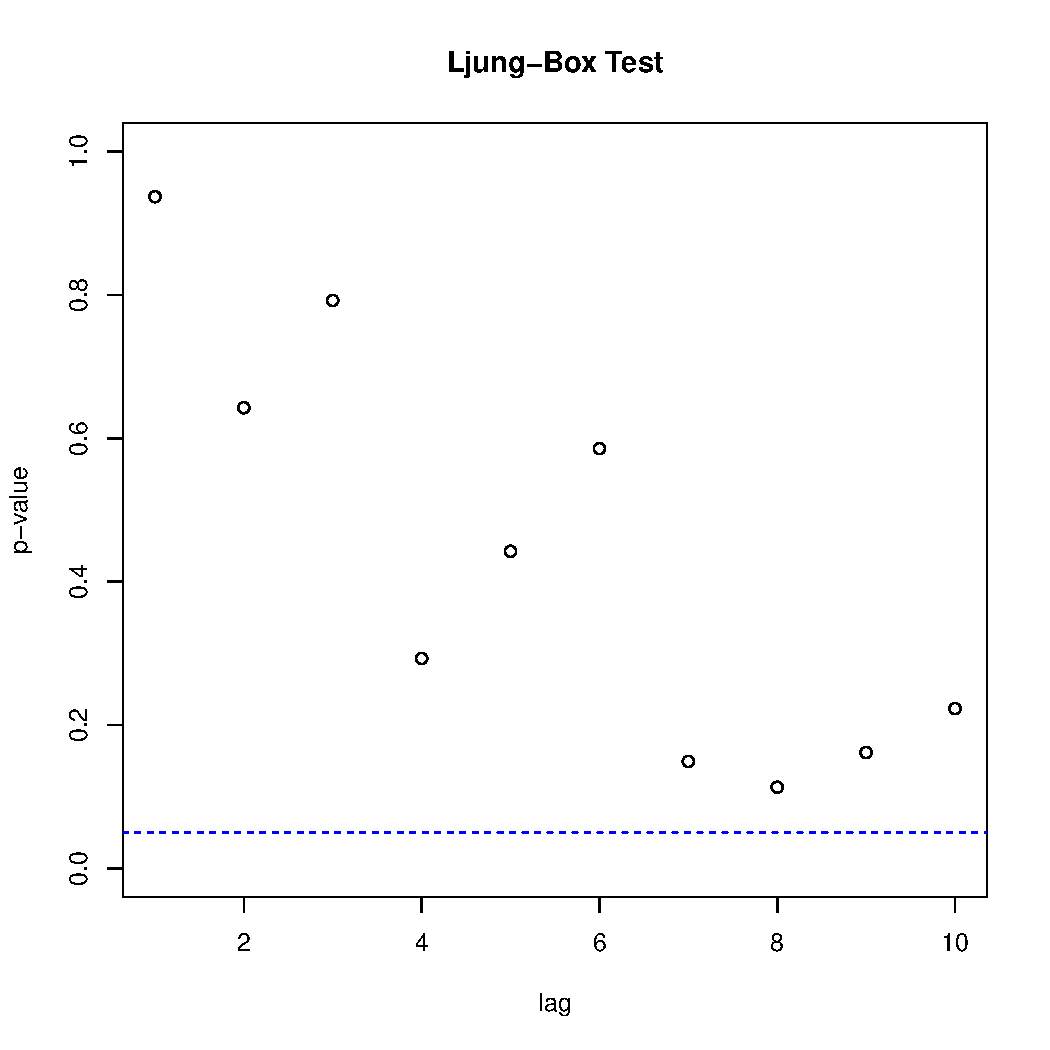
\includegraphics[width=1\linewidth,height=5cm]{images/heap_box.pdf}
%        \caption{}
%        \label{obr:heap_resid_ljung}
    \end{subfigure}
    \caption{Rezíduá odhadnutého \emph{ARIMA} modelu.}
     \label{obr:heap_resid}
\end{figure}

\begin{figure}[H]
    \begin{center}
        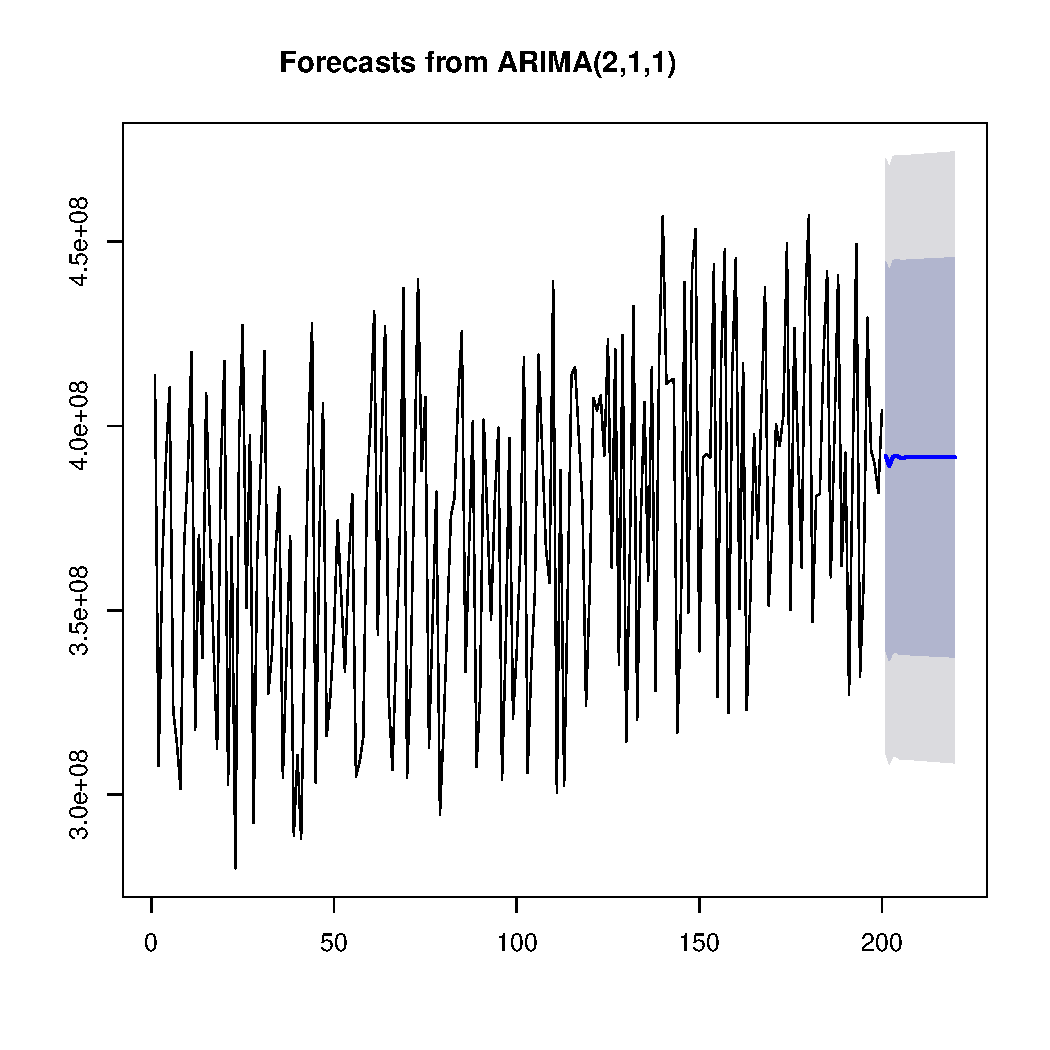
\includegraphics[width=.8\textwidth,height=6cm]{images/heap_forecast.pdf}
        \caption{ARIMA, predikcia na 20 krokov dopredu.}
        \label{obr:heap_forecast}
    \end{center}
\end{figure}

\section{Exponenciálne vyhladzovanie\,--\,Holtova metóda}
Zobecnením dvojitého exponenciálneho vyhladzovania je takzvaná Holtova metóda.
Táto metóda používa dve vyrovnávacie konštanty: $\alpha$ pre vyrovnanie úrovne $l_t$
a $\beta$ pre vyrovnanie smernice $b_t$ (lineárneho trendu).
Výhoda tejto metódy je možnosť použitia v~prúdovom spracovaní, kde nie je možné získať staré hodnoty časovej rady. 
Rovnice majú tvar \ref{exp_holt}. Parametre $\alpha, \beta$ patria do intervalu 
$\alpha,\beta \in (0,1)$. Pre exponenciálne vyhladzovanie platí, 
čím je hodnota parametra $\alpha$ menšia, tým väčšia váha je daná pozorovaniam zo
vzdialenej minulosti.

\begin{eqnarray} \label{exp_holt}
    \hat{y}_{t+h} = l_{t} + hb_{t} \\
    \nonumber l_t = \alpha y_t + (1 - \alpha) (l_{t-1} + b_{t-1}) \\
    \nonumber b_t = \beta (l_t - l_{t-1}) + (1 - \beta)b_{t-1} 
\end{eqnarray}
 
V~jazyku \emph{R} použijeme funkciu \emph{holt}, ktorá počíta predikciu na \emph{k} krokov 
dopredu. Súčasťou funkcie je aj výpočet parametrov $\alpha$~a~$\beta$.

\begin{figure}[H]
    \begin{center}
        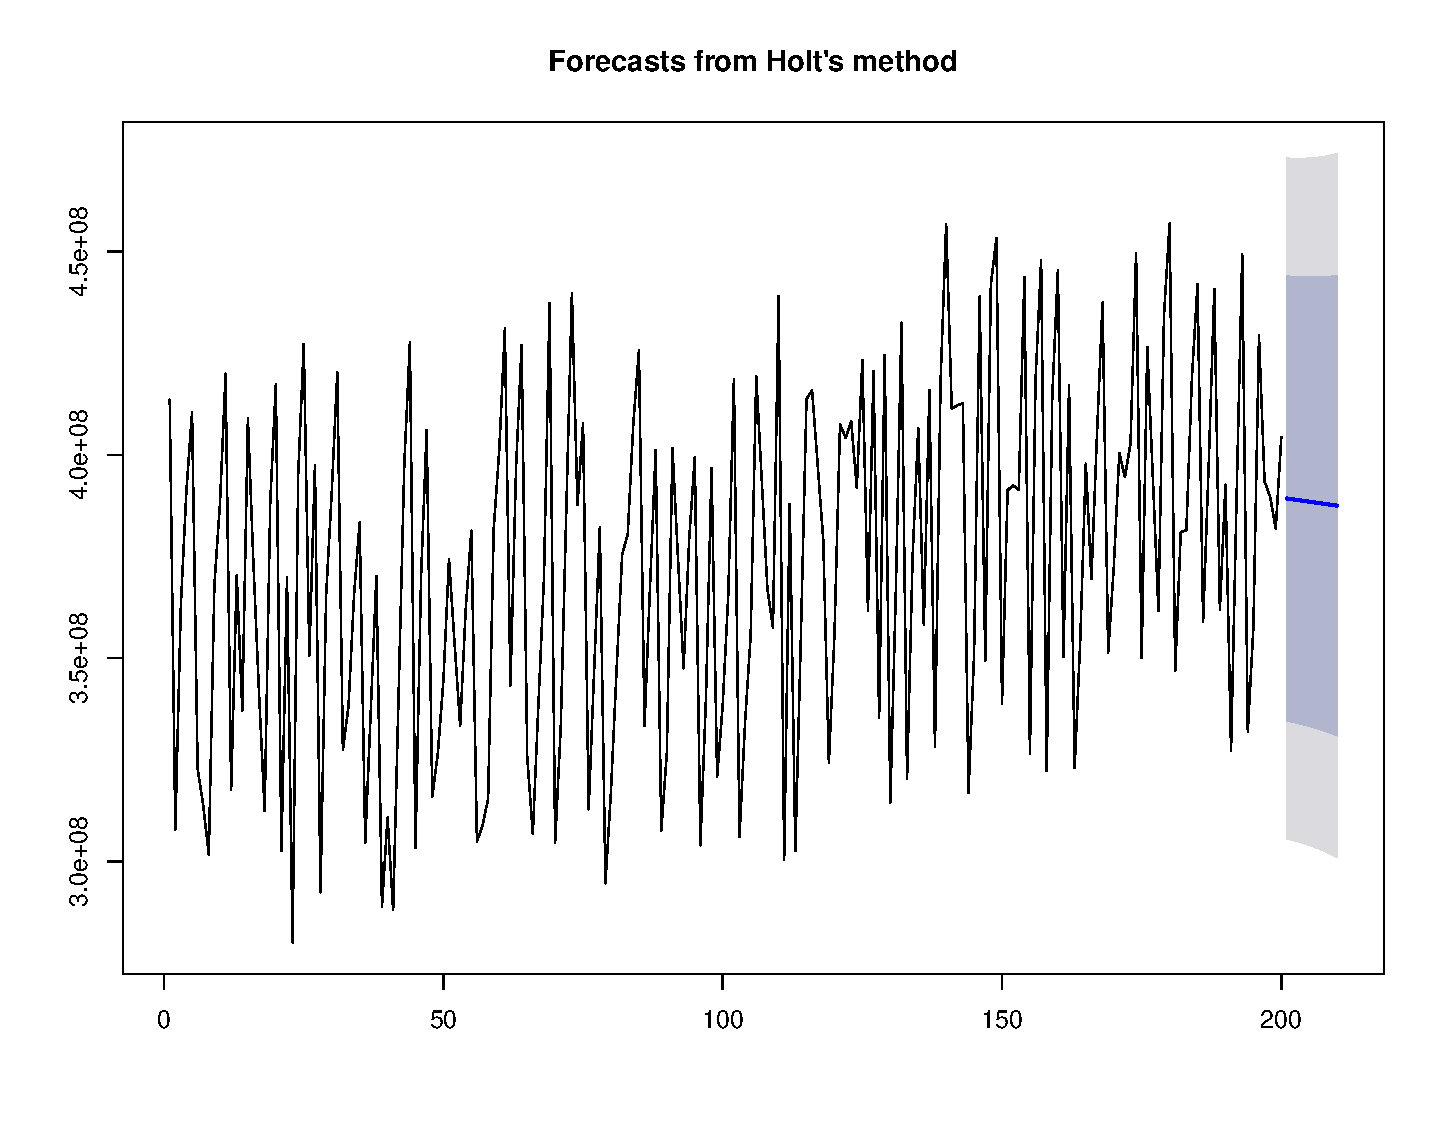
\includegraphics[width=.8\textwidth,height=6cm]{images/heap_holt.pdf}
        \caption{Holt, predikcia na 20 krokov dopredu.}
        \label{obr:heap_holt}
    \end{center}
\end{figure}

\section{Adaptívna filtrácia\,--\,LMS algoritmus}
Odhad parametrov autoregresívneho modelu je možné vypočítať 
pomocou algoritmu \emph{LMS} (Least Mean Square). Výpočet vektoru váh je uvedený
v~rovnici \ref{lms}. Chyba $e$ je rozdiel súčasnej hodnoty časovej rady s~odhadnutou pomocou
váh \emph{LMS}. S~väčším počtom pozorovaní je výpočet váh presnejší. Algoritmus 
má nevýhodu v~tom, že musíme dopredu odhadnúť parameter $\alpha$. Toto býva väčšinou problém 
a preto sa volí buď normalizovaná verzia alebo algoritmus \emph{RLS} (Recursive Least
Square), ktorý tento parameter neobsahuje. V~porovnaní \emph{RLS} algoritmus konverguje
rýchlejšie ale je výpočetne náročnejší.  

\begin{eqnarray} \label{lms}
    w(t+1) = w(t) + \alpha * e(t) * x(t)
\end{eqnarray}

Funkčnosť algoritmu budeme demonštrovať na generovaných dátach, pri ktorých vieme 
aký proces ich generoval. Takto budeme môcť výsledky overiť s~výstupom s~\emph{LMS} algoritmu.

\begin{minipage}{\linewidth}
\begingroup
\fontsize{9pt}{7pt}\selectfont
\begin{verbatim}
n = 1500;
series = arima.sim(n, model=list(ar=c(0.3, -0.8745)), rand.gen=rnorm);
result = lms(series, alpha, AR);
"Estimated weights"
[1]  0.3397577 -0.8287951
\end{verbatim}
\endgroup
\end{minipage}

Z~uvedeného výstupu z~R vidíme že časová rada bola generovaná pomocou \\
\mbox{$y = 0.3*y_{t-1} - 0.8745*y_{t-2}$} a na vstupe boli hodnoty z~normálneho rozdelenia so
strednou hodnotou 0 a~smerodajnou odchýlkou 1. Na grafe \ref{obr:lms} je vidieť priebeh
výpočtu váh v~čase.

\begin{figure}[H]
    \begin{center}
        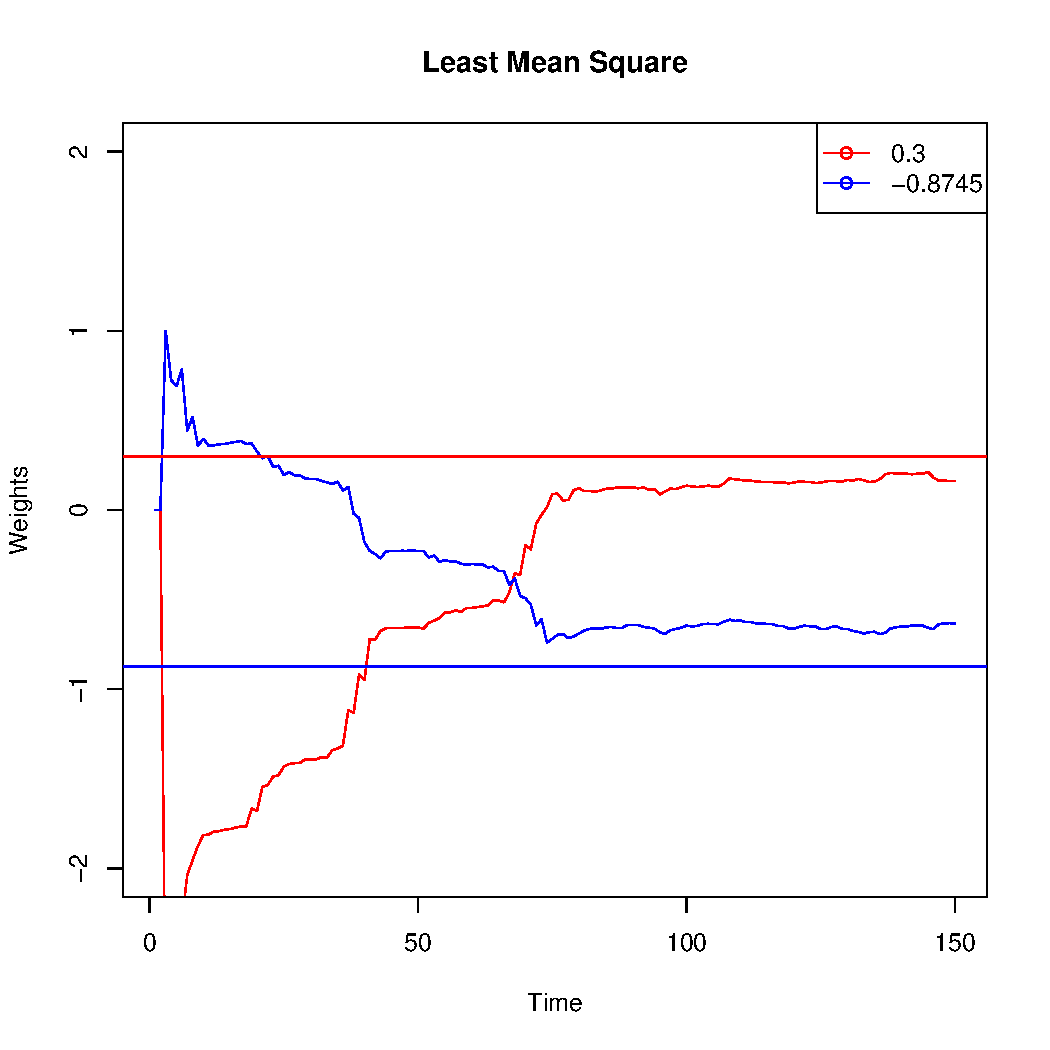
\includegraphics[width=.8\textwidth,height=6cm]{images/lms.pdf}
        \caption{Priebeh výpočtu váh \emph{AR} procesu pomocou \emph{LMS} algoritmu.}
        \label{obr:lms}
    \end{center}
\end{figure}

\section{Záver}
Na záver by som porovnal kvadratickú sumu chýb (\emph{SSE}) oboch modelov. Pre
model \emph{ARIMA} vyšla chyba $3.377059*10^{17}$ a~pre Holtovu metódu $3.657135*10^{17}$. 
Vidíme, že rozdiel nieje významne odlišný. Ak opticky porovnáme grafy \ref{obr:heap_forecast},
\ref{obr:heap_holt} vidíme, že exponenciálne vyhladzovanie strmšie klesá.

Voľba vhodného modelu niekedy nezávisí len na najmenšej chybe predpovedi. Niekedy je nutné
voliť výpočetne nenáročný model, aby bolo možné spracovávať napríklad obrovské množstvo 
časových rád paralelne.

Výsledky adaptívnej filtrácie ukázali, že je možné vypočítať parametre \emph{AR} modelu
pomocou jednoduchých algoritmov ako je napríklad \emph{LMS} ak máme dostatočne veľký počet
pozorovaní. Kombináciou adaptívnej filtrácie a~exponenciálneho vyhladzovania by sme mohli 
dospieť k~zaujímavému modelu, ktorý by mohol mať dobré prediktívne vlastnosti a~nízku
výpočetnu náročnosť.

\section*{Poďakovanie}
Na záver by som chcel poďakovať Ing. Danielovi Němcovi, Ph.D. za návrh na vypracovanie
tejto témy a~za veľmi príjemné a~užitočné konzultácie. Ďalej by som chcel poďakovať Ester
Železňákovej za gramatickú korektúru textu.

\bibliographystyle{czechiso}
\bibliography{bibliography}

%% Pokud nechcete pouzit prilohy, muzete nasledujici radky az po \end{document} smazat
\newpage
\renewcommand{\thesection}{\Alph{section}}
\setcounter{section}{0}
\renewcommand{\thepage}{\roman{page}}
\setcounter{page}{1}

\section{Prílohy}

\begin{itemize}
    \item Zdrojové súbory v~jazyku R v~adresári \texttt{scripts}
    \item Dáta analyzovanej časovej rady v~adresári \texttt{scripts}
    \item Zdrojový text tejto správy v~\LaTeX\,--\,e
\end{itemize}

\end{document}

